\chapter{Applications of Integration}
\section{Area between curves}\begin{enumerate}

\item  How is finding the area under a curve the same as finding the area between 2 curves?  How is it different?

\item You and a friend are comparing homework, and you were assigned a problem to find the area bounded by the two curves $y = x + 1$ and  $
y = x^3  + x^2  - x + 1$.  You found the area of two separate regions and added them together.  Your friend says that whenever there are two regions, you can just find the area of one of them and double it.  Which one of you is correct?

\item  The area between $f(x)$ and $g(x)$ and between $x = a$ and $x = b$ is given by $$\int_a^b {\,\left[ {f(x) - g\left( x \right)} \right]\,dx} $$ (with appropriate assumptions about $f$, $g$, $a$ and $b$).  What happens if either $f$ or $g$ has an $x$-intercept?  Do we need to do anything different?  Why or why not?

\item  The formula $$\int\limits_I {\left[ {f\left( x \right) - g\left( x \right)} \right]\,dx} $$ is supposed to give the area of region that lies between the curves $y = f(x)$ and $y = g(x)$ and ``above'' the interval $I$ on the $x$-axis.  For this formula to work, do $f$ and $g$ both have to be positive functions?  Explain why this works just as well when $g(x) < 0 < f(x)$ and when $g(x) < f(x) < 0$.

\item  Consider the function $f(x) = \cos x$ on $[0, \pi]$ shown in Figure \ref{Chapter6Fig}.  When we find the area bounded by $y = \cos x$, $x = 0$ and $x = \pi$ (shown below) we have to break the calculation into 2 integrals.  Why?  Do we have to do the same thing when we find the average of  $y = \cos x$ on $[0, \pi]$?

 \begin{figure}[ht]
	\centering
		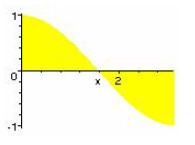
\includegraphics{TeXGraphics/Chapter6Fig.jpg}
	\caption{Area between a curve and the $x$-axis}
	\label{Chapter6Fig}
\end{figure}
 
 
 \end{enumerate}\section{Volumes of revolution}\begin{enumerate}

\item  Consider the region bounded by $y=\sqrt{x}$ and $y=x^2$.  Further, consider two solids:  one where this region is revolved about the $x$-axis and the other where this region is revolved about the $y$-axis.  Finally, consider finding these 2 volumes each in 2 different ways:  in terms of $x$ or in terms of $y$.  Set up all 4 integrals and compare and contrast the methods.

\item Compare and contrast the methods of cylindrical shells, washers and disks.

\item  Verify, using integral methods of finding volumes, that the volume of a right circular cylinder is $$V = \pi r^2 h.$$  

\item  Suppose that the region bounded by $$y = x^3  - 3x - 1$$ and $y = -4$,$-2 \le  x \le  2$, is revolved about $x = 3$.  Explain what would be necessary to compute the volume using the method of washers, and what would be necessary to use the method of cylindrical shells.  Which method would you prefer and why?

\begin{figure}[ht]
	\centering
		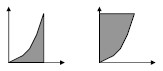
\includegraphics{TeXGraphics/VolRevCom.jpg}
	\caption{Regions to Revolve About Both Axes}
	\label{fig:volrev}
\end{figure}


\item In Figure \ref{fig:volrev} there are two regions.  Each is bounded on one edge by $y=2x^2$ and the point in the upper-right hand corner of each is $(1, 2)$.  Suppose that each region is revolved about each axis to result in 4 different solids.
\begin{enumerate}
\item First, rank the 4 solids in order by size by inspection.
\item Now, check your answer by calculating the volume of all 4 solids.
\item Discuss your ability to predict relative volume.  Observations?
\end{enumerate}


\end{enumerate}\section{Polar curves and areas}\begin{enumerate}

\item  It is easy to algebraically describe and graph spirals using polar coordinates using a polar equation such as $r=\theta$.  Why is this difficult in rectangular coordinates?  Why it is easy in polar coordinates?  How does this reflect on the value of using polar coordinates.

\item  Graph $$r = a\sec \theta $$  for several values of $a$.  What did you find?  Prove that $r=a\sec\theta$ is always a vertical line.  (Hint:  draw a triangle on the polar graph.)   What polar equation will give horizontal lines?  \cite{FWG}

\item  Discuss a procedure for finding the intersection of 2 curves in polar form.  \cite{SBS}  Compare and contrast this method to finding the intersection of 2 curves in rectangular form?

\item  Compare and contrast points given by rectangular coordinates, $(x,y)$, with points given by polar coordinates, $(r, \theta)$.

\item  Compare and contrast the process for finding the area under a curve given in rectangular form and the area enclosed by a polar curve.


\end{enumerate}\section{Arc Length and Surface Area}\begin{enumerate}

\item  What is the formula for finding the length of a segment of a curve $y = f(x)$ on $[a, b]$?  Explain, in general terms, the derivation of this formula.  What hypotheses about $y=f(x)$ must be checked first and what would you do if those hypotheses were not satisfied?


\item  What is the formula for finding the surface area which results from rotating $y = f(x)$ on 
$[a, b]$ about the $y$-axis?  Explain, in general terms, the derivation of either formula.  What hypotheses about $y=f(x)$ must be checked first and what would you do if those hypotheses were not satisfied?

\item Compare and contrast the following 4 formulas:  
\begin{enumerate}
\item  the surface area of $y = f(x)$ revolved about the $x$-axis integrated in term of $x$,
\item  the surface area of $y = f(x)$ revolved about the $x$-axis integrated in term of $y$,
\item  the surface area of $y = f(x)$ revolved about the $y$-axis integrated in term of $x$ and
\item  the surface area of $y = f(x)$ revolved about the $y$-axis integrated in term of $y$,
\end{enumerate} 

\item  Some texts recommend the formula $$L = \int_\alpha ^\beta  {\sqrt {dx^2  + dy^2 } } $$ for the arc length of a smooth curve.  Show that if the function is defined as $y = f(x)$ this formula gives us $$\int_a^c {\sqrt {1 + \left[ {f'\left( x \right)} \right]^2 } dx} $$ and if the function is defined as $x = g(y)$ this formula give us $$\int_b^d {\sqrt {1 + \left[ {g'\left( y \right)} \right]^2 } dy} .$$  Why would $$L = \int_\alpha ^\beta  {\sqrt {dx^2  + dy^2 } } $$ be easier to remember?  How was $$L = \int_\alpha ^\beta  {\sqrt {dx^2  + dy^2 } } $$ derived?

\item  Notice that the integral for arc length of the function $y = f(x)$ on $[a, b]$ is relatively complicated.  I can't just pick any function $y = f(x)$ for you to use on the exam, because I need to have a integral that is ``nice''.  Investigate using 3 elementary functions for $f(x)$ in the arc length formula.  Are the integrals easy to evaluate?

\item  Notice that the integral for the surface area of the function $y = f(x)$ on $[a, b]$ rotated about the $x$-axis is relatively complicated.  I can't just pick any function $y = f(x)$ for you to use on the exam, because I need to have a integral that is ``nice''.  Investigate using 3 elementary functions for $f(x)$ in the surface area formula.  Are the integrals easy to evaluate?

\item  Compare and contrast the formulas for finding the length of an arc of $y = f(x)$ and the formula for finding the surface area of that arc when it is revolved around the $y$-axis.

\end{enumerate}

\section{Work and Centroids}\begin{enumerate}

\item  We have used integrals $\left( {\int\limits_I {f(x)\,dx} } \right)$ to measure length and area and volume, among other measurements.  Why is it possible to use this one mathematical operation to make such diverse measurements with completely different dimensions?

\item  Explain Hooke's Law for springs.  What do we mean by the displacement of a spring?  

\item  Compare and contrast work and force.  If I am holding the calculus book still 4 feet off the floor, is it work or force?  If an elevator moves 3 people from one floor to another, is it work or force?  If a dam is holding water, is it work or force?  

\item  Complete a dimensional analysis on the formula for a centroid of a homogenous lamina.

\item  In general, what does the centroid of a homogeneous lamina represent?  Where is the centroid of a homogeneous circular lamina?  Square lamina?  A lamina that in the shape of an equilateral triangle? 

\item  What type of unit is a joule (i.e., what does it measure)?  What does a joule ``feel'' like?  Find an everyday object and an everyday distance to illustrate what 1 joule ``feels'' like.  Find an everyday activity and measure the number of joules that activity involves.

\item  An integral can be used when we can break an object or situation into ``slices''.  Give 4 distinctly different examples of how we can use the ``slices'' idea in integral applications.

\item  Does the centroid of a lamina with uniform density have to be a point on the lamina?  If the lamina has a line of symmetry, does the centroid have to be a point on the line?

\end{enumerate}
